\documentclass[fleqn,10pt]{wlscirep}
\usepackage[utf8]{inputenc}
\usepackage{pst-all}
\usepackage{hyperref}
\usepackage[hidelinks]{hyperref}
\usepackage{float}
\usepackage{xfrac}
\usepackage{longtable}
\usepackage{subcaption}
\usepackage{multicol}
\usepackage{breqn}
\setlength{\belowcaptionskip}{-0.2cm}
\title{Cryptocurrency Scams}
\let\iif\leftrightarrow
\author[1]{Mateo Restrepo Sierra}
\author[2]{Juan S. C\'ardenas Rodr\'iguez}
\author[3]{David Plazas Escudero}
\affil[1]{Universidad EAFIT, mrestrepos@eafit.edu.co, Student, Medell\'in, Colombia}
\affil[2]{Universidad EAFIT, jscardenar@eafit.edu.co, Student, Medell\'in, Colombia}
\affil[3]{Universidad EAFIT, dplazas@eafit.edu.co, Student, Medell\'in, Colombia}
\keywords{Keyword1, Keyword2, Keyword3}

 \begin{abstract}
	In recent years, cryptocurrencies have become an important part of the financial and economical market all around the world; a big portion of this success is due to their efficient and decentralized transaction system. Even though they were developed for a more trust-worthy financial system, one that does not depend on banks or governments, there have been organizations that had taken advantage of this and other key factors of today's society, such as social media, news, etc. In this paper, we approach the transaction system of cryptocurrencies using system dynamics for a more wide study of how this currencies can increase their price only with a constant flow of investors and transactions. A dynamic hypothesis and Forrester diagram were constructed after defining some relationships between the variables that were considered relevant in the system. The model was validated and some policies were proposed in order to achieve some limits in the prices of cryptocurrencies.
 \end{abstract}
\begin{document}

\flushbottom
\maketitle

\thispagestyle{empty}

\section{Introduction}
In the 1920s, Charles Ponzi duped investors when he convinced them that he will return a 50\% revenue every 90 days; he was actually paying the old investors with the money given by the new ones. This is known as the Ponzi Scheme nowadays; since the virtual currencies lack of regulation and have enhanced privacy for trading, they can be and are being used by fraudsters to perpetrate their frauds in similar fashion \cite{ponzi}.

\noindent In 2017, the cryptocurrency company BitConnect launched its new coin BitConnect Coin (BCC, not to be confused with BitCoin Cash), which assured every user that whatever investment they made in their currency and made part of their loan and exchange platform (which allowed them to loan the company USD and Bitcoin to the company in favor of some interests) they will return up to 40\% of their initial investment every month. After using broad marketing strategies to avoid their investors to know about their fraudulent intentions and recollecting thousands of investments, they closed the loan and exchange platform; so, all the people who invested in the BCC lost all their money because of the 96\% drop in the price of the coin. Even the company promised to return some money for the people who got affected by given them the average of the price of the coin in the last 15 days but, given that BCC was at such a low price there were several financial lossess by the investors. In this day and age, there are new companies like XRPConnect, EthConnect, Bunny Token and NEOConnect that are replicating the schemes that BCC made without any type of regulation which, as what happened with BitConnect, can lead to disastrous results \cite{nextWeb}.

\noindent In this manner, cryptocurrencies can over-inflate their price by artificially manipulating the price by marketing it with unrealistic expectations so people start buying the coin and in some delay, selling it to other people to obtain profit through the Exchanges or the Peer to Peer system, who would put more coins in the market through mining. As they exploit the price and people invest more in the coin, they then can abuse this by incrementing by a big margin their Exchange rate or, on the other side, the company changes the coins it possesses for USD or another currency and, proceed to devaluate their coin so they do not have to pay people back. \cite{bcc11}.

\noindent On the other hand, price leveraging is not as hard in cryptocurrencies as other stocks that are available in the market. An article written in the Journal of Monetary Economics about the price manipulation in the bitcoin system, that the sudden spike in the price of bitcoin in 2013 happened due to suspicious activity in an exchanges called ``Mt.Gox Bitcoin Currency Exchange'', which 600000 BTC valued at 188 million USD were acquiered using bots, artificially inflating the price without any real substance; the article explains how this could have a massive effect in the growth rate of BTC in a positive manner, reaching a 4\% growth rate each day after \cite{PMitBE}.

\subsection{Problem of cryptocurrencies}
Taking account of all the above, the cryptocurrency system allows for people to abuse it in fraudulent ways to augment the growth rate of the price of that coin without any type of repercusion, due to the lack of goverment regulation. On the other hand, as an articles of forbes says, most of investors in this currencies like this investment because of the same lack of government involvement \cite{forbes}. In this manner, nowadays companies like Bunny Token, ETH Connect, XRPConnect and mire are expecting 1\% growth in their price daily without any type of proof or security for the investors without too much control because, of the lack of control they have, leading to a easier atmosphere to scam people.

\indent To conclude, it's important to notice that even if the problem and the variables have a very short span, there can be found a lot of documentation about them because they were one of the trending topics last year. Most people see Bitcoin and other cryptocurrencies as a safe economic investment and a way to make easy profit. Although we are not saying that is something that we should thrive to eliminate completely, it is important to examine how this system works and start to make policies that makes investing in this opportunity a safer place for the consumer and, stop catastrophes like BitConnect to don't ever happen again.



\section{Important Concepts}
\begin{itemize}
\item Ponzi Scheme: Is a fraudulent type of investment scheme that uses later investments to provided quick, high returns to early investors. These schemes focus on attracting new investors rather than engaging in any legitimate investment. In the 1920s, Charles Ponzi initially bought a small number of international mail coupons in support of his scheme, but quickly switched to using incoming funds from new investors to pay returns to earlier investors. While dealing with international exchange rates, postal organizations and foreign currency kept him from producing actual revenue, the scheme did allow him to brag and advertise about the investment opportunity. In a few months, he managed to convince hundreds of people to invest in his business; Ponzi used the funds to buy a mansion and deposited cash in banks all across New England (today UK) \cite{ponzi} \cite{ezubao}.

\item Foreign Exchange Market: Global online network where traders buy or sell currencies, its main objective is to set the exchange rate for currencies \cite{foreignExchange}. The basic concept behind the foreign exchange (or forex) market is for trading currencies,
one pair against another. In 2010, it was the world’s largest market, consisting of almost \$2 trillion in daily volume and is growing rapidly. The price of each currency within the pair is determined by a number of factors, such as changes in political leadership, economic booms or busts or even natural disasters \cite{forex}. 

\item ICO (Initial coin offering): It is a method in which a cryptocurrency startup firm sells a number of its cryptocurrency to companies and investors to back their project up; it is similar to A IPO (initial public offering), where new companies sell shares to other companies or investors. Early investors in the operation are usually motivated to buy the cryptocoins in the hope that the plan becomes successful after it launches which could translate to a higher cryptocurrency value than what they purchased it for before the project was initiated. Since these fund-raising operations are not regulated by financial authorities, although there are successful ICOs, there are ICOs and crowd-sales campaigns that are fraudulent. Funds that are lost due to fraudulent activities may never be recovered \cite{ICO}.
\item Blockchain Protocol: It is used to serialize transactions of the currency among its users, it is maintained by a replicated state machine that keeps user's transactions and balances. This state machine is managed by nodes, called miners. Cryptographic methods are used to ensure security on each transaction, the miners commit the transactions into a global-decentralized log called blockchain. This is the protocol that several cryptocurrencies use for their trades and transactions \cite{blockchain}.
\end{itemize}


\section{Analysis of the problem and variables identification}
\subsection{Scope of the problem}
To approach the problem of this article, it is necessary to understand how the dynamic of buying and selling coins through the exchanges can affect the price of that specific cryptocurrency; at the same time, it is important to notice how goverment regulation can affect the price, so we can thoroughly determine how effective will goverment taxes affect the system.

\subsection{Model purpose}
Understand how the cryptocurrency buying-selling dynamic through exchanges, can increase growth rate and affect the price altogether. Therefore, understanding how fraudelent schemes can leverage this system exponentially and artificially manipulate the price.

\subsection{Variables identification and historical background}
We identified 10 variables that affect the problem of over inflating this types of currencies for scams. These are:
\begin{enumerate}
	\item Price of the cryptocurrency (CC): this is the market value in US dollars that the actual coin has. Measurement units: \$ USD
    \item Number of CC bought: is the number of CC bought by the users through the Exchanges. Measurement units: dimensionless.
    \item Number of CC sold: is the number of CC sold by the users to the Exchange company for another currency. Measurement units: Dimensionless.
    \item Investors: is the number of investors that have invested on the coin or the company releasing it. Measurement units: dimensionless.
    \item Number of Exchanges: this is the number of Exchanges that trade this specific CC. Measurement units: dimensionless.
   	\item Volatility: it's the uncertainty in percentage of, given a value of winning fee, how much one can lose or win in relation to that fee. Measurement units: \%
    \item Earnings: this is on average how much a given person earns by trading this CC. Measurement units: \$ USD
    \item Exchange fees: this is the fee that the Exchange uses in every trade you make with their rates. Measurement units: \$ USD
    \item Government taxes: this is the taxes that the government applies to the Exchange. Measurement units: \$ USD
    \item Growth rate: It refers to the price of the cryptocurrency divided by time\cite{GR}. Measurement units: USD/Time.
\end{enumerate}

\noindent In order to give some historical background of these variables, we are going to use the BitConnect example because, although there exists several companies who work in a similar fashion, this is the only one in this span of time that has completed the scam completely. It is important to notice that, finding measurements of variables such as the CC sold and bought can be a real hard task because the number of transactions per day with this coin considerably big; and, although we could check the blockchain for every single operation in each CC, it is something to improve upon in the future with an algorithm that does this automatically.

\noindent In this manner, instead of measuring the CC sold and bought will find the historical background of the Volume of the CC which represents the amount of money in USD that has been traded of that CC every 24 hours; even if is not exactly the same as the variables mentioned, we could have a good knowledge of this variables through that graph. Figure \ref{img-trading} shows trading data on BitConnect.
\begin{figure}[H]
	\centering
    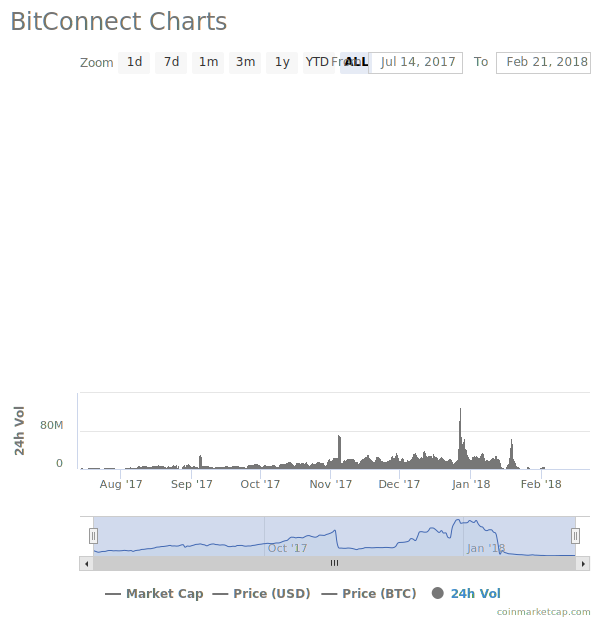
\includegraphics[scale=0.8]{files/Trading.pdf}
    \caption{Trading data on BitConnect.}
    \label{img-trading}
\end{figure}

\noindent On the other hand, the same occurs when we try to find the number of investors; it would be something impossible to find at exact quantity of how much investors are investing in the CC. So, instead, we can find the graph of the Market Cap that is the number of investors multiplied the price of a unitary action of the company. In this way, we would get a very good grasp of the behavior of this variable. Figure \ref{img-marketcap} shows said data.

\begin{figure}[H]
	\centering
    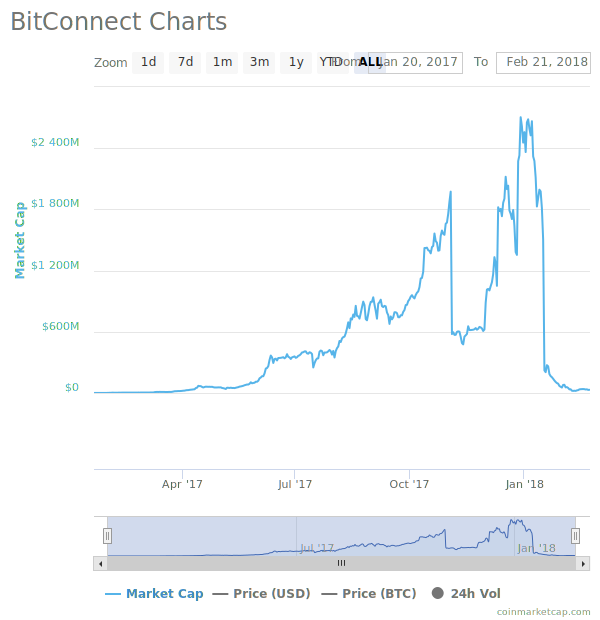
\includegraphics[scale=0.7]{files/Market_Cap.pdf}
    \caption{Market cap data on BitConnect.}
    \label{img-marketcap}
\end{figure}

\noindent Finally, the price of the CC is the easiest to find, as it is documented in a wide variety of websites. Figure \ref{img-pricebcc} shows the price of the BitConnect Coin.

\begin{figure}[H]
	\centering
    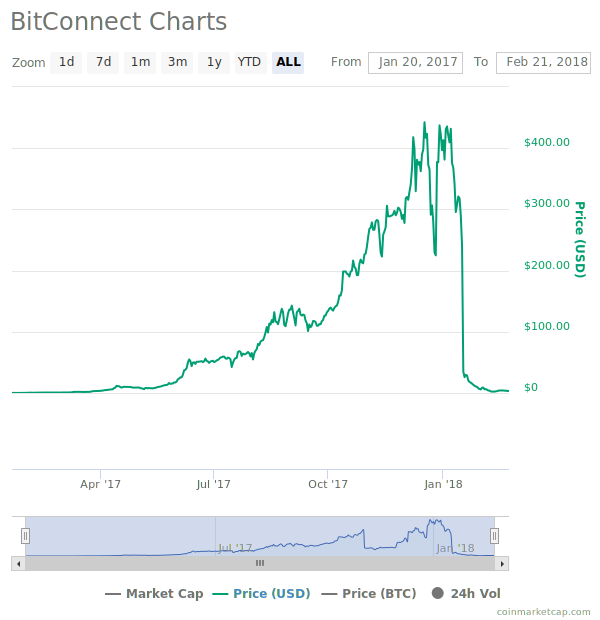
\includegraphics[scale=0.7]{files/Price_bCC.pdf}
    \caption{Price on BitConnect Coin.}
    \label{img-pricebcc}
\end{figure}

This data was obtained from Coin Market Cap on \cite{cmc}.

\section{Dynamic hypothesis}
\subsection{Causal loop diagram}
Figure \ref{img:causalloop} shows the causal loop diagram for the model in study.
\begin{figure}[H]
	\centering
    \includegraphics[scale=0.75]{files/CausalLoopDiagram.pdf}
    \caption{Causal loop diagram for cryptocurrency exchange market.}
    \label{img:causalloop}
\end{figure}


\section{Forrester diagram}
The time scope selected for the simulation was 4 years (48 months for Vensim), this is due to the fact that the exchange market, in general, is highly volatile and unpredictable; it would be a mistake to attempt a larger simulation. Besides, for the kind cryptocurrency that is being modeled, the price tends to increase in a short period of time. The complete Forrester Diagram is shown in Figure \ref{img:forrester}.
\begin{figure}[ht]
	\centering
    \includegraphics[scale=0.6]{files/ForresterDiag.pdf}
    \caption{Forrester diagram for cryptocurrency exchange market.}
    \label{img:forrester}
\end{figure}

It is important to highlight that, in comparison with the dynamic hypothesis, the Forrester Diagram has a considerably more variables; this is due to the fact that, during the construction of aforementioned diagram, we considered more calculations and relations between than the variables defined in first place. Although, the dynamic hypothesis has the general system behavior. This diagram was developed in Vensim.

\section{Model Validation}
\subsection{Units Consistency}
The units check validation is shown in Figure \ref{img:units}
\begin{figure}[H]
	\centering
    \includegraphics[scale=0.3]{files/Units.png}
    \caption{Units check in Vensim}
    \label{img:units}
\end{figure}
Though, it must be noted that the units check approval was achieved using some parameters, this proves that some of the equations proposed for the model are not the best options, even though they are consistent with whether the dependency was proportional or inversely proportional. 
\subsection{Stress Test}
	The variables selected for the stress test are CC Bought and New Investors. They were set as follows:
	\begin{multicols}{2}
    \begin{itemize}
    \item CCBought$=0$
    \columnbreak 
    \item NewInvestors$=0$
    \end{itemize}
		
	\end{multicols}
	
	\subsubsection{CC Bought}
		Setting the number of cryptocurrencies bought as zero, would imply an important drop in the price, this is shown in Figure \ref{img:extrprice}. This shows that the model behaves correctly after changing CCBought. 
        \begin{figure}[H]
        	\centering
            \includegraphics[scale=0.3]{files/ExtrPrice.pdf}
            \caption{Price after setting CCBought as zero.}
            \label{img:extrprice}
        \end{figure}
        On the other hand, it is important to note that the growth rate also behaves accordingly, as it is shown in Figure \ref{img:extrgrowth}. This is because it settles after a few months, which proves that it depends on the price change and it if it does not change, the growth rate will be constant.
        
        \begin{figure}[H]
        	\centering
            \includegraphics[scale=0.3]{files/ExtrCCBoughtGrowth.pdf}
            \caption{Growth rate behavior for CCBought as zero.}
            \label{img:extrgrowth}
        \end{figure}
        
	\subsubsection{New Investors}
    	Setting the number of new investors as zero, implies that there will not be new buyers and the market would, kind of, get stuck with the same people. As the cryptocurrency market needs people to invest and them being in a constant flow, the price of the CC would drop after a few months. This was achieved during this test, as shown in Figure \ref{img:extrinvprice}
        \begin{figure}[H]
        	\centering
            \includegraphics[scale=0.3]{files/ExtrInvestPrice.pdf}
            \caption{Results for price after setting the new investors as zero.}
            \label{img:extrinvprice}
		\end{figure}
        Same for the growth rate, which proves accordingly the behavior, shown in Figure \ref{img:extrinvgrowth}.
        \begin{figure}[H]
        	\centering
            \includegraphics[scale=.3]{files/ExtrInvestGrowth.pdf}
            \caption{Results for Growth Rate for zero new investors.}
            \label{img:extrinvgrowth}
        \end{figure}

\section{Policies}
\subsection{Base Model}
	Before the policies for addressing the problem are presented, it is necessary to show that, indeed, there is a problem and that it can be seen in the model constructed. For this, the base model will be presented, with results for both price and growth rate.

	The results for the base model test are shown in Figure \ref{img:base}, for both price (a) and growth rate (b).
	\begin{figure}[H]
      \centering
      \begin{subfigure}[t]{0.4\textwidth}
        \includegraphics[scale = 0.3]{files/BasePrice.pdf}
        \centering
        \caption{Results for price.}
      \end{subfigure}
      \hspace{1cm}
      \begin{subfigure}[t]{0.4\textwidth}
        \includegraphics[scale = 0.3]{files/BaseGrowth.pdf}
        \centering
        \caption{Results for growth rate.}
      \end{subfigure}
      \caption{Base model test.}
      \label{img:base}
	\end{figure}
    
   It can be noted that the plot of price (Figure \ref{img:base}.a) for the base model is similar to Figure \ref{img-pricebcc}, which shows price of BitConnect Coin; showing a significant growth in the price of the CC in a very short time period. The problem that is going to be addressed is attempting to limit this growth or, at least, extend the time that the market needs to reach similar prices. A possible improvement to control the system using the model, can be through two specific variables: taxes and investors. 
   
   \subsection{Policies: Government Taxes to Exchanges}
   The first one is controlling the trading in the exchanges, this may be achieved through the government imposing taxes to the exchanges; as the exchanges have to pay to the government, they have to augment their own taxes (exchange fees), so this will represent a change in the price and obviously in the growth rate, as is shown in Figure \ref{img:polittaxes}.
   
   \begin{figure}[H]
      \centering
      \begin{subfigure}[t]{0.4\textwidth}
        \includegraphics[scale = 0.3]{files/politTaxesPrice.pdf}
        \centering
        \caption{Results for price.}
      \end{subfigure}
      \hspace{1cm}
      \begin{subfigure}[t]{0.4\textwidth}
        \includegraphics[scale = 0.3]{files/politTaxesGrowth.pdf}
        \centering
        \caption{Results for growth rate.}
      \end{subfigure}
      \caption{Results after setting government taxes.}
      \label{img:polittaxes}
	\end{figure}
   Note that the growth rate keeps a normal fluctuation and that the price is oscillating and tending to drop, as well as the price maximum is around 175USD, whereas the base model was around 480USD; this shows that the policy is effective and changes are taking place in the model results.
   
   
   \subsection{Policies: Limit the Number of New Investors}
   one of the most important factors that rise the price of a cryptocurrency is the number of investors that a certain cryptocurrency can handle a great amount of people. In this order, it is of the utmost importance to regulate the number of  investors that can enter the system monthly so the price grows in a more balanced way. Therefore, we tested the system allowing only ten thousand people maximum to enter the system per month; in the real system, is not that hard to control this aspect but it needs government regulation to make it achievable. The results of this policy can be observed in Figure \ref{img:politinv}
   
    \begin{figure}[H]
      \centering
      \begin{subfigure}[t]{0.4\textwidth}
        \includegraphics[scale = 0.3]{files/politInvPrice.pdf}
        \centering
        \caption{Results for price.}
      \end{subfigure}
      \hspace{1cm}
      \begin{subfigure}[t]{0.4\textwidth}
        \includegraphics[scale = 0.3]{files/politInvGrowth.pdf}
        \centering
        \caption{Results for growth rate.}
      \end{subfigure}
      \caption{Results after limit in New Investors.}
      \label{img:politinv}
	\end{figure}

\section{CONCLUSIONS}
It was successfully analyzed the received data, using statistical tests which allowed to fit data to use in the simulation, find auto-correlation and test homogeneity between data. It is important to remark that in the fitting of the data the distributions have a left bias as most of the times are positive and close to zero.

It was successfully implemented the simulation model in Python, which partially represents the Neuromédica pharmacy medicine retriveal system. The model did not fully validate with the tests done, which presents an important limitation of the implemented model; even though, the results given are not useful for the real system, this article proposes a methodology for solving this types of problems. 

For further work, a model using continuous simulation could be used as the inter-arrival times are so close to zero that the system could be analyzed supposing a continuous flux of patients. Also, a graphical user interface can be done so it is easily explained without the use of code.
%Bibs
\bibliographystyle{ieeetran}
\bibliography{ref}


\end{document}
